% Akulin--Karlov. Batch 02, revision v2. Source: R36 CP02 and original scans.
% Editable geometry: source semantics first; no raster is embedded in this drawing.
\documentclass[border=5pt]{standalone}
\usepackage{fontspec,unicode-math}
\setmainfont{Noto Serif}
\setsansfont{Noto Sans}
\setmathfont{STIXTwoMath-Regular.otf}
\usepackage{tikz}
\usetikzlibrary{arrows.meta,calc,intersections,decorations.markings}
\definecolor{ScienceInk}{HTML}{000000}
\definecolor{ScienceCurve}{HTML}{000000}
\tikzset{
 axis/.style={draw=ScienceInk,line width=.70pt,-{Latex[length=2.2mm,width=1.25mm]}},
 baseline/.style={draw=ScienceInk,line width=.70pt},
 trace/.style={draw=ScienceCurve,line width=1.8pt,line cap=round,line join=round},
 level/.style={draw=ScienceInk,line width=2.1pt,line cap=butt},
 virtual/.style={draw=ScienceInk,line width=1.15pt,dash pattern=on 4pt off 3pt},
 photon/.style={draw=ScienceCurve,line width=1.05pt,-{Latex[length=2.25mm,width=1.35mm]},line cap=round},
 channel/.style={draw=ScienceCurve,line width=1.05pt,-{Latex[length=2.25mm,width=1.35mm]},line cap=round},
 dim/.style={draw=ScienceInk,line width=.70pt,-{Latex[length=1.8mm,width=1.1mm]}},
 lab/.style={text=ScienceInk,font=\fontsize{15}{18}\selectfont,inner sep=2pt},
 ticklab/.style={text=ScienceInk,font=\fontsize{13}{16}\selectfont\itshape,inner sep=1pt},
 levlab/.style={text=ScienceInk,font=\fontsize{14}{17}\selectfont,inner sep=2pt},
 panel/.style={text=ScienceInk,font=\fontsize{16}{19}\selectfont\itshape,inner sep=1pt}}
\pagestyle{empty}
\begin{document}

% CP08 reviewed against R36 lecture 9, pp. 91-92: E_{n,K}=E_n+K*hbar*omega.
% Heights are SCHEMATIC: no calibrated experimental line spacings are implied.
% Three near-resonant levels are E_1,0 ; E_2,-1 ; E_3,-2.
% CP08 preserves every printed stroke and index, while restoring short gaps at
% the two arrow/level contacts where arrows are dimension indicators.
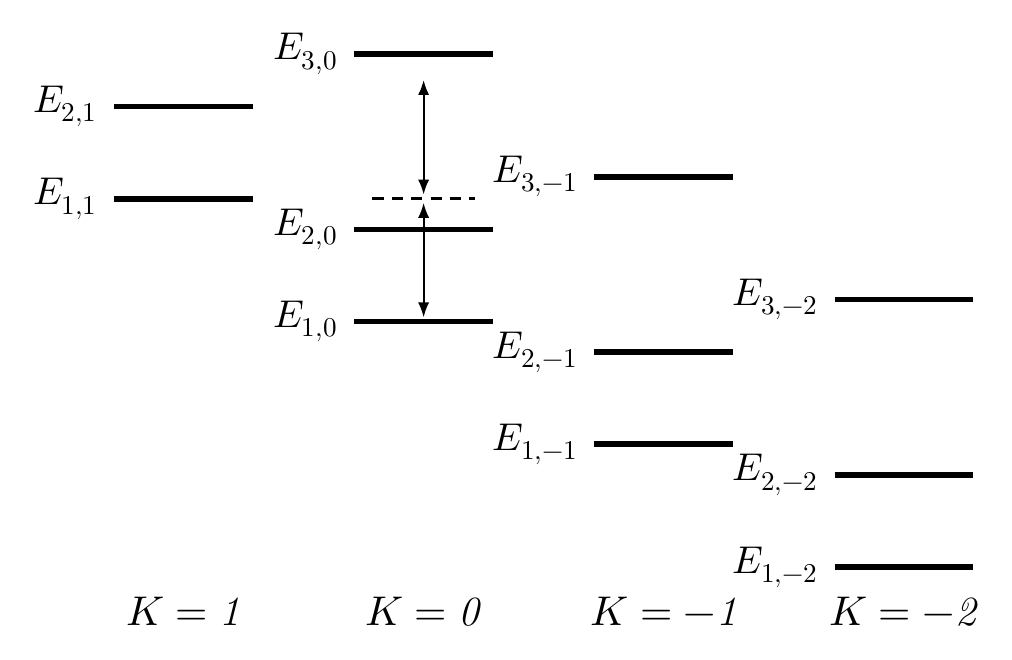
\begin{tikzpicture}[x=1cm,y=1cm]
\def\Eone{0}\def\Etwo{.75}\def\Ethree{2.18}\def\Photon{1}\def\Es{1.56}\def\Ybase{3.50}
% State anchors are derived from the single spectral model.
\foreach \k/\xc/\col in {1/1.85/P,0/4.90/Z,-1/7.95/M,-2/11.0/N}{
 \foreach \n/\e in {1/\Eone,2/\Etwo,3/\Ethree}{
  \pgfmathsetmacro\yy{\Ybase+\Es*(\e+\k*\Photon)}
  \coordinate (L\n\col) at (\xc,\yy);
  % E3,+1 is outside the original viewport and is not invented in this panel.
  \ifnum\k=1\ifnum\n=3\else
   \draw[level] ({\xc-.88},\yy)--({\xc+.88},\yy);
   \node[levlab,anchor=east] at ({\xc-1.0},\yy) {$E_{\n,\k}$};
  \fi\else
   \draw[level] ({\xc-.88},\yy)--({\xc+.88},\yy);
   \node[levlab,anchor=east] at ({\xc-1.0},\yy) {$E_{\n,\k}$};
  \fi
 }
 \node[lab,anchor=north] at (\xc,.08) {$K=\mathit{\k}$};
}
\coordinate (V1) at (4.9,{\Ybase+\Es*\Photon});
\coordinate (V2) at (4.9,{\Ybase+2*\Es*\Photon});
% Restored displaced dashed reference, NOT the E2,0 solid line.
\draw[virtual] ($(V1)+(-.65,0)$)--($(V1)+(.65,0)$);
\draw[baseline,shorten >=1.5pt,shorten <=1.5pt,{Latex[length=1.9mm]}-{Latex[length=1.9mm]}] (L1Z)--(V1);
\draw[baseline,shorten >=1.5pt,shorten <=1.5pt,{Latex[length=1.9mm]}-{Latex[length=1.9mm]}] (V1)--(V2);
\end{tikzpicture}

\end{document}
